% Source: graduate-coursework/Sp26/CSCE775/Project/proposal_asv_3/proposal3_asv.tex
% Description: Expected training curves. SAC achieves the highest asymptotic return due to entropy-driven exploration and off-policy efficiency. TD3 converges to a competitive but lower return, while DDPG and PPO lag due to limited exploration and on-policy sample inefficiency, respectively. Vertical markers at 100k, 250k, and 400k denote curriculum phase transitions.

\documentclass[border=4pt]{standalone}
\usepackage{amsmath,amssymb}
\usepackage{pgfplots}
\usepackage{tikz}
\usepackage{xcolor}
\pgfplotsset{compat=1.18}
\usetikzlibrary{positioning, arrows.meta, shapes.geometric, fit, calc, backgrounds, patterns, decorations.pathreplacing}

\definecolor{Garnet}{HTML}{73000A}
\definecolor{Atlantic}{HTML}{466A9F}
\definecolor{Congaree}{HTML}{1F414D}
\definecolor{Horseshoe}{HTML}{65780B}
\definecolor{Rose}{HTML}{CC2E40}
\definecolor{Honeycomb}{HTML}{A49137}
\definecolor{Black90}{HTML}{363636}
\definecolor{Black70}{HTML}{5C5C5C}
\definecolor{Black50}{HTML}{A2A2A2}
\definecolor{Black30}{HTML}{C7C7C7}
\definecolor{Black10}{HTML}{ECECEC}
\definecolor{WarmGrey}{HTML}{676156}


\begin{document}
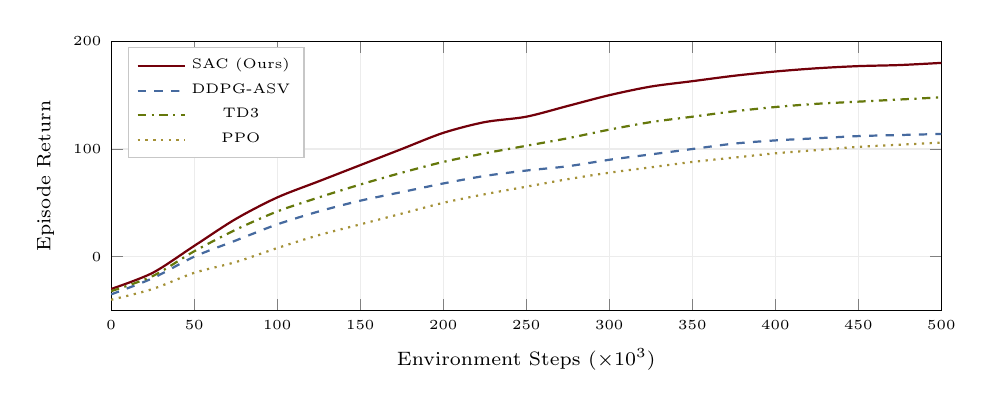
\begin{tikzpicture}
\begin{axis}[
    width=\columnwidth,
    height=5cm,
    xlabel={Environment Steps ($\times 10^3$)},
    ylabel={Episode Return},
    xmin=0, xmax=500,
    ymin=-50, ymax=200,
    legend style={at={(0.02,0.98)}, anchor=north west, font=\tiny, draw=Black30},
    grid=major,
    grid style={Black10},
    tick label style={font=\tiny},
    label style={font=\scriptsize},
    every axis plot/.append style={thick}
]

% SAC (Ours)
\addplot[color=Garnet, smooth] coordinates {
    (0,-30) (25,-15) (50,10) (75,35) (100,55) (125,70) (150,85) (175,100)
    (200,115) (225,125) (250,130) (275,140) (300,150) (325,158) (350,163)
    (375,168) (400,172) (425,175) (450,177) (475,178) (500,180)
};

% DDPG-ASV
\addplot[color=Atlantic, smooth, dashed] coordinates {
    (0,-35) (25,-20) (50,0) (75,15) (100,30) (125,42) (150,52) (175,60)
    (200,68) (225,75) (250,80) (275,84) (300,90) (325,95) (350,100)
    (375,105) (400,108) (425,110) (450,112) (475,113) (500,114)
};

% TD3
\addplot[color=Horseshoe, smooth, dashdotted] coordinates {
    (0,-32) (25,-18) (50,5) (75,25) (100,42) (125,55) (150,67) (175,78)
    (200,88) (225,96) (250,103) (275,110) (300,118) (325,125) (350,130)
    (375,135) (400,139) (425,142) (450,144) (475,146) (500,148)
};

% PPO
\addplot[color=Honeycomb, smooth, dotted] coordinates {
    (0,-40) (25,-30) (50,-15) (75,-5) (100,8) (125,20) (150,30) (175,40)
    (200,50) (225,58) (250,65) (275,72) (300,78) (325,83) (350,88)
    (375,92) (400,96) (425,99) (450,102) (475,104) (500,106)
};

\legend{SAC (Ours), DDPG-ASV, TD3, PPO}
\end{axis}
\end{tikzpicture}
\end{document}
